\chapter{Fundamentos de lattice Boltzmann}
\label{chap:fundamentos}

El origen del m\'etodo de lattice Boltzmann est\'a directamente vinculado a los aut\'omatas celulares, una discretizaci\'on del espacio con celdas individuales que conviven en un estado particular, y que actualizan su estado en cada paso de tiempo de acuerdo a reglas que tienen en cuenta el estado de las celdas vecinas. El estudio sistem\'atico de los aut\'omatas celulares inspir\'o, a trav\'es de los LGCA (\emph{lattice gass cellular automaton}), una de las primeras aplicaciones en la simulaci\'on de fluidos. La evoluci\'on continua del m\'etodo, que implic\'o una transformaci\'on de la mec\'anica booleana a otra de caracter\'isticas continuas, con la consecuente eliminaci\'on de ruido estad\'istico y de la falta de invariancia de Galileo, deriv\'o en la concepci\'on moderna de LB.
\nomenclature[A]{LB}{Lattice Boltzmann}

De manera simult\'anea, a partir de los trabajos de Luo \cite{luo_unified_1998} y Lallemand y Luo \cite{lallemand_theory_2000}, se demostr\'o que el m\'etodo de LB puede derivarse de la ecuaci\'on de Boltzmann continua, y por lo tanto corresponde a una discretizaci\'on especial de la misma. La aplicaci\'on de t\'ecnicas multiescala como la expansi\'on de Chapman-Enskog, desarrolladas para analizar la ecuaci\'on de Boltzmann original, facilit\'o el descubrimiento del v\'inculo formal con la din\'amica macrosc\'opica reproducida.

Este \'ultimo camino aporta una base s\'olida para comprender, utilizar y expandir el m\'etodo de LB como t\'ecnica num\'erica de resoluci\'on de ecuaciones diferenciales en derivadas parciales. Por lo tanto, en el presente cap\'itulo se detallan las caracter\'isticas principales de esta idea, mostrando c\'omo es posible obtener una ecuaci\'on de lattice Boltzmann a partir de la ecuaci\'on de Boltzmann continua. Por simplicidad, los conceptos desarrollados est\'an principalmente relacionados con el an\'alisis de modelos hidrodin\'amicos e isot\'ermicos, pero contienen los fundamentos matem\'aticos necesarios para comprender los modelos detallados en los cap\'itulos siguientes. Para mayores detalles, se recomienda la consulta de los libros de Kr\"uger \cite{kruger_lattice_2017} y Succi \cite{succi_lattice_2018}.
\newpage

\section{Naturaleza cin\'etica del m\'etodo}
\label{sec:kinetic}
La descripci\'on matem\'atica de la din\'amica de fluidos se basa tradicionalmente en la hip\'otesis de un medio continuo, con escalas temporales y espaciales suficientemente mayores que las asociadas a la naturaleza atom\'istica subyacente. En este contexto, suelen encontrarse referencias a descripciones microsc\'opicas, mesosc\'opicas o macrosc\'opicas. La descripci\'on microsc\'opica, por un lado, hace referencia a una descripci\'on molecular, mientras que la macrosc\'opica involucra una visi\'on continua completa, con cantidades tangibles como densidad o velocidad del fluido. Por otro lado, entre ambas aproximaciones se encuentra la teor\'ia cin\'etica mesosc\'opica, la cu\'al no describe el movimiento de part\'iculas individuales, sino de distribuciones o colecciones representativas de dichas part\'iculas.
\par
La variable fundamental de la teor\'ia cin\'etica se conoce como funci\'on de distribuci\'on de part\'iculas (en ingl\'es \emph{particle distribution function} o PDF), que puede verse como una generalizaci\'on de la densidad $\rho$ y que a su vez tiene en cuenta la velocidad microsc\'opica de las part\'iculas \bxi{}. Por lo tanto, mientras que $\rho(\bm{x},t)$ representa la densidad de masa en el espacio f\'isico, la funci\'on de distribuci\'on \fvar{} corresponde a la densidad de masa tanto en el espacio f\'isico como en el espacio de velocidades.
\nomenclature[A]{\fdp{}}{Funci\'on de distribuci\'on de part\'iculas o \emph{particle distribution function}}
\nomenclature[N]{$\rho$}{Densidad}
\nomenclature[N]{$E$}{Energ\'ia total}
\nomenclature[N]{$\bm{u}$}{Velocidad macrosc\'opica}
\nomenclature[N]{$\bm{x}$}{Coordenada espacial}
\nomenclature[N]{$t$}{Tiempo}
\nomenclature[N]{$\xi$}{Velocidad microsc\'opica de part\'iculas}
\par
La funci\'on de distribuci\'on $f$ se relaciona con variables macrosc\'opicas como densidad $\rho$ y velocidad $\bm{u}$ a trav\'es de momentos, es decir, integrales de $f$ con funciones de peso dependientes de \bxi{} sobre todo el espacio de velocidades. En particular, la densidad de masa macrosc\'opica puede obtenerse como el momento de orden cero, es decir:
\begin{equation}
	\rho(\bm{x},t) = \int f(\bm{x},\bm{\xi},t) \, \mbox{d}^3 \xi,
\end{equation}
en el cual se considera la contribuci\'on de part\'iculas con todas las velocidades posibles en la posici\'on $\bm{x}$ a tiempo $t$. Por otro lado, la densidad de impulso y las densidades de energ\'ia total ($E$) e interna ($e$) pueden determinarse mediante momentos de primer y segundo orden:
\begin{equation}
	\rho(\bm{x},t) \bm{u}(\bm{x},t) = \int \bm{\xi} f(\bm{x},\bm{\xi},t) \, \mbox{d}^3 \xi,
\end{equation}
\begin{equation}
	\rho(\bm{x},t) E(\bm{x},t) = \dfrac{1}{2} \int |\bm{\xi}|^2 f(\bm{x},\bm{\xi},t) \, \mbox{d}^3 \xi,
\end{equation}
\begin{equation}
	\rho(\bm{x},t) e(\bm{x},t) = \dfrac{1}{2} \int |\bm{\xi}-\bm{u}|^2 f(\bm{x},\bm{\xi},t) \, \mbox{d}^3 \xi.
\end{equation}


\subsection{Funci\'on de distribuci\'on de equilibrio}
En el an\'alisis original realizado para gases diluidos y monoat\'omicos, Maxwell \red{cita} menciona que cuando un gas permanece sin perturbaciones por un per\'iodo de tiempo suficientemente largo, la funci\'on de distribuci\'on \fvar{} alcanza una distribuci\'on de equilibrio \feqvar{} (\emph{equilibrium distribution function} o EDF por sus siglas en ingl\'es), que es isotr\'opica en el espacio de velocidades en torno a $\bm{\xi} = \bm{u}$. En este caso, si se toma un marco de referencia que se desplaza con velocidad $\bm{u}$, entonces dicha \edf{} puede expresarse como $f^{eq}(\bm{x},|\bm{v}|,t)$. Por otro lado, si se supone que la \edf{} puede expresarse de forma separable como producto de funciones unidimensionales:
\nomenclature[A]{EDF}{Funci\'on de distribuci\'on de equilibrio o \emph{equilibrium distribution function}}

\begin{equation}
	f^{eq}(|\bm{v}|^2) = f^{eq}(v_x^2 + v_y^2 + v_z^2)=f_{1D}^{eq}(v_x^2) \, f_{1D}^{eq}(v_y^2) \, f_{1D}^{eq}(v_z^2),
\end{equation}
entonces puede demostrarse que dicha distribuci\'on queda definida como:

\begin{equation}
	f^{eq}(\bm{x},|\bm{v}|^2,t) = \mbox{e}^{3a}\mbox{e}^{b|\bm{v}|^2}.
\end{equation}
Como las colisiones de part\'iculas monoat\'omicas conservan masa, impulso y energ\'ia, pueden encontrarse las constantes $a$ y $b$ imponiendo que $f^{eq}(\bm{x},|\bm{v}|,t)$ posea los mismos momentos que $f(\bm{x},|\bm{v}|,t)$. De esta manera, se puede etablecer una expresi\'on expl\'icita para la \edf{}:
\begin{equation}
	f^{eq}(\bm{x},|\bm{v}|,t) 
	= \rho \left( \dfrac{3}{4\pi e} \right)^{3/2} \mbox{e}^{-3|\bm{v}|^2/(4e)}
	= \rho \left( \dfrac{1}{2\pi RT} \right)^{3/2} \mbox{e}^{-|\bm{v}|^2/(2RT)}.
\end{equation}

En este caso se utiliz\'o la relaci\'on de gases ideales
\begin{equation}
	\rho e = \frac{3}{2}\rho RT=\frac{3}{2}p,
\end{equation}
donde $R$ es una constante, $p$ representa a la presi\'on y $T$ a la temperatura macrosc\'opica del fluido.
\nomenclature[N]{$R$}{Constante de gases ideales}
\nomenclature[N]{$T$}{Temperatura macrosc\'opica}
\nomenclature[N]{$p$}{Presi\'on}


\subsection{La ecuaci\'on de Boltzmann}
\label{sec:ec_boltz}
La funci\'on de distribuci\'on \fvar{} establece propiedades tangibles de un fluido a trav\'es de sus diferentes momentos. Asimismo, es posible determinar una ecuaci\'on que permita modelar su evoluci\'on en el espacio f\'isico, de velocidades, y el tiempo. En el an\'alisis siguiente, se omitir\'a la dependencia de $f$ con $(\bm{x}, \bm{\xi}, t)$ por claridad.
\par
Como $f$ es una funci\'on de la posici\'on $\bm{x}$, de la velocidad de las part\'iculas \bxi{}, y del tiempo $t$, la derivada total de $f$ respecto al tiempo resulta:

\begin{equation}
	\dfrac{df}{dt} = \left( \dfrac{\partial f}{\partial t} \right) \dfrac{dt}{dt}
	               + \left( \dfrac{\partial f}{\partial x_{\beta}} \right) \dfrac{dx_{\beta}}{dt}
	               + \left( \dfrac{\partial f}{\partial \xi_{\beta}} \right) \dfrac{d\xi_{\beta}}{dt}.
\end{equation}

Este diferencial total puede reescribirse usando la definici\'on de la velocidad de las part\'iculas ($dx_{\beta}/dt = \xi_{\beta}$), e incorporando una fuerza volum\'etrica $\bm{F}$ determinada por la segunda ley de Newton mediante $d\xi_{\beta}/dt = F_{\beta}/\rho$. Si se utiliza la notaci\'on tradicional $\Omega (f) = df/dt$ para el diferencial total respecto al tiempo se obtiene una expresi\'on para describir la evoluci\'on de $f$, conocida como ecuaci\'on de Boltzmann:

\begin{equation}
	\dfrac{\partial f}{\partial t}  +  \xi_{\beta} \dfrac{\partial f}{\partial x_{\beta}}            +  \dfrac{F_{\beta}}{\rho} \dfrac{\partial f}{\partial \xi_{\beta}} =\Omega(f).
	\label{eq:boltz}
\end{equation}

La \eq{eq:boltz} puede verse como una ecuaci\'on de advecci\'on para $f$, donde los dos primeros t\'erminos del miembro izquierdo corresponden a la advecci\'on de $f$ con la velocidad de part\'iculas \bxi{}, mientras que el tercero representa el efecto de las fuerzas externas sobre la FDP. Por otro lado, el miembro derecho contiene un t\'ermino de fuente conocido como operador de colisi\'on, que representa la redistribuci\'on local de $f$ debido a colisiones entre las propias part\'iculas. Estas colisiones conservan masa, momento y energ\'ia, lo que se traduce en restricciones para los momentos de $\Omega$:
\begin{subequations}
	\begin{align}
		\int \Omega(f) \, \mbox{d}^3 \xi = 0 \\
		\int \bm{\xi} \, \Omega(f) \, \mbox{d}^3 \xi = \bm{0} \\		
		\int |\bm{\xi}|^2 \, \Omega(f) \, \mbox{d}^3 \xi = 0 	
	\end{align}
	\label{eq:omega_restrict}
\end{subequations}


\subsection{Ecuaciones de conservaci\'on macrosc\'opicas}
\label{sec:cons_macro}
Las ecuaciones de conservaci\'on de propiedades macrosc\'opicas pueden obtenerse como momentos de la ecuaci\'on de Boltzmann, es decir, multiplicando la \eq{eq:boltz} por funciones de \bxi{} e integrando sobre todo el espacio de velocidades. Para simplificar este an\'alisis, es necesario introducir previamente una notaci\'on general para los distintos momentos de $f$:

\begin{subequations}
	\begin{equation}
		\Pi_0 = \int f \, \mbox{d}^3 \xi = \rho
	\end{equation}
	\begin{equation}
		\Pi_{\alpha} = \int \xi_{\alpha} f \, \mbox{d}^3 \xi = \rho u_{\alpha}
	\end{equation}
	\begin{equation}
		\Pi_{\alpha \beta} = \int \xi_{\alpha} \xi_{\beta} f \, \mbox{d}^3 \xi
	\end{equation}
	\begin{equation}
		\Pi_{\alpha \beta \gamma} = \int \xi_{\alpha} \xi_{\beta} \xi_{\gamma} f \, \mbox{d}^3 \xi
	\end{equation}
	\label{eq:f_moments}
\end{subequations}

La ecuaci\'on m\'as simple de obtener corresponde a la de conservaci\'on de masa. Integrando la \eq{eq:boltz} en el espacio de velocidades, y usando las \eqs{eq:omega_restrict}{eq:f_moments}, se obtiene:

\begin{equation}
	\dfrac{\partial \rho}{\partial t} + \dfrac{\partial (\rho u_{\beta})}{\partial x_{\beta}} = 0.
\end{equation}

De manera similar, multiplicando la \eq{eq:boltz} por $\xi_{\alpha}$ e integrando en el espacio de velocidades se obtiene la ecuaci\'on de conservaci\'on de impulso lineal:

\begin{equation}
	\dfrac{\partial \rho u_{\alpha}}{\partial t} + \dfrac{\partial \Pi_{\alpha \beta}}{\partial x_{\beta}} = F_{\alpha},
	\label{eq:mom_flux}
\end{equation}
donde $\Pi_{\alpha \beta}$ se define como el tensor de flujo de impulso. Si se descompone la velocidad de las part\'iculas como $\bm{\xi} = \bm{u} + \bm{v}$, entonces la \eq{eq:mom_flux} puede reescribirse como

\begin{equation}
	\dfrac{\partial \rho u_{\alpha}}{\partial t} 
	+ \dfrac{\partial (\rho u_{\alpha} u_{\beta})}{\partial x_{\beta}} = 
	\dfrac{\partial \sigma_{\alpha \beta}}{\partial x_{\beta}} + F_{\alpha}.
	\label{eq:impulso}
\end{equation}
donde $\sigma_{\alpha \beta}$ representan un tensor de tensiones:

\begin{equation}
	\sigma_{\alpha \beta} = -\int v_{\alpha} v_{\beta} f \, \mbox{d}^3 \xi
\end{equation}

Finalmente, puede seguirse un procedimiento similar para encontrar una ecuaci\'on macrosc\'opica de conservaci\'on de energ\'ia. Multiplicando la \eq{eq:boltz} por $\xi_{\alpha} \xi_{\beta}$ e integrando en el espacio de velocidades se obtiene:

\begin{equation}
	\dfrac{\partial \rho E}{\partial t} + \dfrac{1}{2} \dfrac{\Pi_{\alpha\alpha\beta}}{\partial x_{\beta}} = F_{\beta} u_{\beta}.
	\label{eq:energy_flux}
\end{equation}

Por otro lado,  si se descompone el momento como en la ecuaci\'on de conservaci\'on de impulso y usando la \eq{eq:impulso} multiplicada por $u_{\alpha}$, la \eq{eq:energy_flux} puede reescribirse como:

\begin{equation}
	\dfrac{\partial \rho e}{\partial t} + \dfrac{(\rho u_{\beta} e)}{\partial x_{\beta}} = \sigma_{\alpha\beta} \dfrac{\partial u_{\alpha}}{\partial x_{\beta}} - \dfrac{\partial q_{\beta}}{\partial x_{\beta}},
\end{equation}
donde el flujo de calor $\bm{q}$ est\'a definido por el momento

\begin{equation}
	q_{\beta} = \dfrac{1}{2} \int v_{\alpha} v_{\alpha} v_{\beta} f \, \mbox{d}^3 \xi
\end{equation}


En este punto es interesante destacar que si bien la convervaci\'on de masa queda definida exactamente, las ecuaciones de impulso y energ\'ia dependen de la forma de $f$, que todav\'ia no es conocida. Por ejemplo, en el caso particular en que $f \simeq f^{eq}$, las ecuaciones de conservaci\'on se convierten en las ecuaciones de Euler para impulso y energ\'ia:

\begin{subequations}
	\begin{equation}
	 	\dfrac{\partial \rho u_{\alpha}}{\partial t} 
	  + \dfrac{\partial (\rho u_{\alpha} u_{\beta})}{\partial x_{\beta}} 
	  =	-\dfrac{\partial p}{\partial x_{\alpha}} + F_{\alpha} ,	
	\end{equation}
	\begin{equation}
		\dfrac{\partial \rho e}{\partial t} 
	  + \dfrac{(\rho u_{\beta} e)}{\partial x_{\beta}} 
	  = -p \dfrac{\partial u_{\beta}}{\partial x_{\beta}}.
	\end{equation}
	\label{eq:macro_euler}	
\end{subequations}

Este hecho muestra que los procesos macrosc\'opicos de disipaci\'on viscosa y difusi\'on de calor se encuentran directamente vinculados a la desviaci\'on de $f$ respecto de su valor de equilibrio, y constituye un concepto fundamental en la comprensi\'on de la forma final de la t\'ecnica num\'erica. 



\section{Discretizaci\'on del espacio de velocidades} 
El desarrollo mostrado en la \se{sec:kinetic} destaca la posibilidad de representar adecuadamente el comportamiento de un fluido usando una funci\'on de distribuci\'on \fvar{}. Sin embargo, dicha distribuci\'on se encuentra definida en un espacio con 7 dimensiones, es decir, 3 coordenadas espaciales, 3 para el espacio de velocidades, y una para el tiempo, de modo que la resoluci\'on de ecuaciones en este espacio multidimensional involucra un esfuerzo computacional considerable. Por otro lado, es necesario considerar que este enfoque no es siempre justificable, porque en definitiva son los momentos de la ecuaci\'on de Boltzmann (integrales en el espacio de velocidades) los que conducen a ecuaciones macrosc\'opicas de conservaci\'on de masa, impulso y energ\'ia. 
\par 
Estas caracter\'isticas originaron la b\'usqueda de versiones simplificadas de la ecuaci\'on de Boltzmann que no sacrifiquen el comportamiento macrosc\'opico, es decir, de sus momentos. Entre estas alternativas es posible encontrar las expansiones en base al n\'umero de Mach \cite{he_lattice_1997} o en series de Hermite \cite{shan_kinetic_2006}. Si bien ambas conducen a la misma representaci\'on de Navier-Stokes, la representaci\'on en series de Hermite presenta una base matem\'atica m\'as s\'olida, y es la que se detallar\'a a continuaci\'on.
\par
La idea fundamental de la espansi\'on usando polinomios de Hermite consiste en simplificar la \edf{} $f^{eq}$ y discretizar el espacio de velocidades, pero manteniendo las leyes de conservaci\'on macrosc\'opicas. En particular, como $f^{eq}$ tiene una forma exponencial conocida, puede ser expresada a trav\'es de la funci\'on generatriz de estos polinomios (tambi\'en exponencial), mientras que los momentos de masa e impulso son representados como integrales de $f^{eq}$ multiplicadas por los polinomios de Hermite. Estas caracter\'isticas permiten, por un lado, encontrar una expresi\'on reducida de $f^{eq}$ a trav\'es de una suma truncada de polinomios de Hermite, mientras que se conservan adecuadamente los primeros momentos. Por otro lado, esta representaci\'on permite evaluar dichos momentos mediante sumas discretas donde el integrando est\'a evaluado en coordenadas espec\'ificas $\bm{\xi}_i$, llamadas absisas. Estas t\'ecnicas pueden extenderse a la representaci\'on de la funci\'on de distribuci\'on $f$.


\subsection{Adimensionalizaci\'on}
Antes de proceder con la discretizaci\'on de $f$ y $f^{eq}$ en series de Hermite, es conveniente reescribir las ecuaciones governantes de forma adimensional, con el objetivo de simplificar los pasos siguientes.
\par
La funci\'on de distribuci\'on \fvar{} representa la densidad de masa en el espacio f\'isico tridimensional y en el espacio de velocidades, tambi\'en tridimensional. Por lo tanto, las unidades de $f$ en el SI son:
\begin{equation}
	[f] = \mbox{kg} \times \dfrac{1}{\mbox{m}^3} \times \dfrac{1}{(\mbox{m/s})^3} = \dfrac{\mbox{kg} \, \mbox{s}^3}{\mbox{m}^6}.
\end{equation}

Las propiedades de un fluido pueden analizarse en t\'erminos de una longitud caracter\'istica $l$, una velocidad caracter\'istica $V$ y una densidad caracter\'istica $\rho_0$. Si se denota con * a las cantidades adimensionales, entonces es posible escribir los operadores diferenciales adimensionales como:
\begin{equation}
\dfrac{\partial}{\partial t^*} = \dfrac{l}{V}\dfrac{\partial}{\partial t}, \qquad
\dfrac{\partial}{\partial x^*} = l\dfrac{\partial}{\partial x}, \qquad
\dfrac{\partial}{\partial \xi^*} = V\dfrac{\partial}{\partial \xi}.
\end{equation}
\nomenclature[N]{$l$}{Longitud caracter\'istica}
\nomenclature[N]{$V$}{Velocidad caracter\'istica}
\nomenclature[N]{$\rho_0$}{Densidad caracter\'istica o de referencia}

Esto lleva a escribir a la forma adimensional de la ecuaci\'on de Boltzmann en $d$ dimensiones:
\begin{equation}
	\dfrac{\partial f^*}{\partial t^*}  
	+  \xi^*_{\alpha} \dfrac{\partial f^*}{\partial x^*_{\alpha}} 
	+  \dfrac{F^*_{\alpha}}{\rho^*} \dfrac{\partial f^*}{\partial \xi^*_{\alpha}} =\Omega^*(f^*),
	\label{eq:boltz_adim}
\end{equation}
donde $f^* = fV^d/\rho_0$, $\bm{F}^* = \bm{F}l/(\rho_0 V^2)$, $\rho^2 = \rho/\rho_0$ y $\Omega^*= \Omega l V^2 / \rho_0$. Siguiendo el mismo procedimiento, la funci\'on de equilibrio adimensional resulta:
\begin{equation}
	f^{eq*}	= \left( \dfrac{\rho^*}{2\pi \theta^*} \right)^{d/2} \mbox{e}^{-(\bm{\xi}^* - \bm{u}^*)^2/(2\theta^*)}
\end{equation}

En este caso, $\theta^*$ corresponde a la temperatura adimensional $\theta^*=RT/V^2$. En las secciones siguientes se trabajar\'a exclusivamente con cantidades adimensionales, omitiendo el super\'indice * por claridad.


\subsection{Expansi\'on en series de Hermite}
Las bases de la teor\'ia cin\'etica muestran que el operador de colisi\'on preserva ciertos momentos de la funci\'on de distribuci\'on, lo que a su vez implica que los momentos de $f^{eq}$ y $f$ deben coincidir:
\begin{subequations}
	\begin{align}
		\int f(\bm{x},\bm{\xi},t) \, \mbox{d}^3 \xi &=& \int f^{eq}(\rho, \bm{u},\theta,\bm{\xi}) \, \mbox{d}^3 \xi &=& \rho(\bm{x},t)\\
		\int f(\bm{x},\bm{\xi},t) \bm{\xi}\, \mbox{d}^3 \xi &=& \int f^{eq}(\rho, \bm{u},\theta,\bm{\xi}) \bm{\xi}\, \mbox{d}^3 \xi &=& \rho(\bm{x},t)\bm{u}(\bm{x},t)\\
		\int f(\bm{x},\bm{\xi},t) \dfrac{|\bm{\xi}|^2}{2} \, \mbox{d}^3 \xi &=& \int f^{eq}(\rho, \bm{u},\theta,\bm{\xi}) \dfrac{|\bm{\xi}|^2}{2} \, \mbox{d}^3 \xi &=& \rho(\bm{x},t)E(\bm{x},t)\\		
		\int f(\bm{x},\bm{\xi},t) \dfrac{|\bm{\xi}-\bm{u}|^2}{2} \, \mbox{d}^3 \xi &=& \int f^{eq}(\rho, \bm{u},\theta,\bm{\xi}) \dfrac{|\bm{\xi}-\bm{u}|^2}{2} \, \mbox{d}^3 \xi &=& \rho(\bm{x},t)e(\bm{x},t)		
	\end{align}
	\label{eq:cons_moments}	
\end{subequations}

Las cantidades conservadas de la \eq{eq:cons_moments} pueden obtenerse como integrales de $f$ o $f^{eq}$ en el espacio de velocidades. Por lo tanto, la expansi\'on en series de Hermite contribuye a transformar esas integrales continuas en sumas discretas evaluadas en puntos espec\'ificos del espacio de velocidades.
\par
Los polinomios de Hermite se definen en un espacio $d$-dimensional como: \cite{shan_kinetic_2006,grad_kinetic_1949}
\begin{equation}
	\bm{H}^{(n)} (\bm{x})= (-1)^n\dfrac{1}{\omega (\bm{x})} \bm{\nabla}^{(n)}\omega(\bm{x}),
\end{equation}
donde $\omega(\bm{x})$ es una funci\'on generatriz:
\begin{equation}
	\omega(\bm{x}) = \dfrac{1}{(2\pi)^{d/2}}\mbox{e}^{-\bm{x}^2/2}
\end{equation}

Tanto $\bm{H}^{(n)}$ como $\bm{\nabla}^{(n)}$ son tensores de rango $n$, de modo que sus $d^n$ componentes pueden expresarse como $H^{(n)}_{\alpha_1 \ldots \alpha_n}$ y $\nabla^{(n)}_{\alpha_1 \ldots \alpha_n}$, donde $\{\alpha_1 \ldots \alpha_n\}$ son \'indices comprendidos entre $1$ y $d$. Para el caso particular de una dimensi\'on, los polinomios se reducen a
\begin{equation}
	H^{(n)}(x)=(-1)^{(n)} \dfrac{1}{\omega(x)} \dfrac{d^n}{dx^n}\omega(x), \qquad 
	\omega(x) = \dfrac{1}{\sqrt{2\pi}}\mbox{e}^{-x^2/2}
\end{equation}

Los polinomios de Hermite son ortogonales respecto a la funci\'on de peso $\omega(\bm{x})$ y constituyen una base completa en $\Re^n$ \cite{wiener_fourier_1989}, de modo que es posible representar cualquier funci\'on $f(\bm{x})$ suficientemente suave mediante:
\begin{equation}
	f(\bm{x}) = \omega(\bm{x}) \sum_{n=0}^{\infty}\dfrac{1}{n!}\bm{a}^{(n)} \cdot \bm{H}^{(n)}(\bm{x}), \qquad 
	\bm{a}^{(n)} = \int f(\bm{x})\bm{H}^{(n)}(\bm{x}) d^nx
\end{equation}

Esta propiedad permite aplicar la expansi\'on en series de Hermite a la \edf{} en el espacio de velocidades
\begin{subequations}
	\begin{equation}
		f^{eq}(\rho, \bm{u}, \theta, \bm{\xi}) = \omega(\bm{\xi}) \sum_{n=0}^{\infty}\dfrac{1}{n!}\bm{a}^{(n)eq}(\rho, \bm{u}, \theta) \cdot \bm{H}^{(n)}(\bm{\xi})
	\end{equation}
	\begin{equation}
		\bm{a}^{(n)eq}(\rho, \bm{u}, \theta) = \int f^{eq}(\rho, \bm{u}, \theta, \bm{\xi})\bm{H}^{(n)}(\bm{\xi}) \mbox{d}^d \xi
	\end{equation}
	\label{eq:feq_hermite}
\end{subequations}

En particular, puede verse que la \edf{} tiene la misma forma funcional que la funci\'on generatriz $\omega(\bm{x})$:
\begin{equation}
	f^{eq}(\rho, \bm{u}, \theta, \bm{\xi}) = \dfrac{\rho}{\theta^{d/2}} \, \omega \left( \dfrac{\bm{\xi} - \bm{u}}{\sqrt{\theta}} \right),
\end{equation}
de modo que el c\'alculo de los coeficientes $\bm{a}^{(n)}$ puede simplificarse mediante:
\begin{equation}
	\bm{a}^{(n)eq} = \rho \int \omega(\bm{\eta})\bm{H}^{(n)}(\sqrt{\theta}\bm{\eta} - \bm{u}) \mbox{d}^d \eta,
\end{equation}
donde $\bm{\eta} = (\bm{\xi} - \bm{u})/\sqrt{\theta}$. El c\'alculo de estas integrales puede realizarse directamente, de modo que los primeros coeficientes resultan:
\begin{subequations}
	\begin{align}
		a^{(0),eq}          &= \rho              \\ 
		a^{(1),eq}_{\alpha} &= \rho u_{\alpha}   \\
		a^{(2),eq}_{\alpha\beta} &= \rho \left[ u_{\alpha} u_{\beta} + (\theta-1)\delta_{\alpha\beta} \right]   \\
		a^{(3),eq}_{\alpha\beta\gamma} &= \rho \left[ u_{\alpha} u_{\beta} u_{\gamma} + (\theta-1)(\delta_{\alpha\beta}u_{\gamma} + \delta_{\beta\gamma}u_{\alpha} + \delta_{\gamma\alpha}u_{\beta}) \right].
	\end{align}
	\label{eq:eq_coeffs}
\end{subequations}

A partir de la \eq{eq:eq_coeffs} puede observarse que los coeficientes de la serie de Hermite est\'an directamente relacionados con las principales cantidades conservadas. En esta l\'inea, puede demostrarse que existe una relaci\'on similar para los coeficientes de la expansi\'on en series de Hermite de la funci\'on de distribuci\'on $f$:
\begin{subequations}
	\begin{align}
		a^{(0),eq} &= \int f^{eq} \mbox{d}^d \xi  &= \rho  &= \int f \mbox{d}^d \xi &= a^{(0)}   \\ 
		a^{(1),eq}_{\alpha} &= \int \xi_{\alpha}f^{eq} \mbox{d}^d \xi  &= \rho u_{\alpha}  &= \int \xi_{\alpha}f \mbox{d}^d \xi &= a^{(1)}_{\alpha}   \\ 		
		\dfrac{a^{(2),eq}_{\alpha\alpha}+\rho d}{2} &= \int \dfrac{|\bm{\xi}|^2}{2} f^{eq} \mbox{d}^d \xi  &= \rho E  &= \int \dfrac{|\bm{\xi}|^2}{2} f \mbox{d}^d \xi &= \dfrac{a^{(2)}_{\alpha\alpha}+\rho d}{2}
	\end{align}
\end{subequations}

La representaci\'on adecuada de las leyes de conservaci\'on macrosc\'opica puede alcanzarse con pocos t\'erminos de las series de Hermite, aunque se ha observado que la inclusi\'on de t\'erminos de mayor orden contribuyen a mejorar la precisi\'on y estabilidad del m\'etodo num\'erico final \cite{dhumieres_multiple-relaxation-time_2002}. De esta forma, la representaci\'on en serie de $f^{eq}$ con s\'olo $N=3$ t\'erminos puede aproximarse por:
\begin{equation}
\begin{aligned}
	f^{eq} &\approx \omega(\bm{\xi}) \sum_{n=0}^{N=3} \dfrac{1}{n!}\bm{a}^{(n),eq} \cdot \bm{H}^{(n)}(\bm{\xi}) \\
	&\approx \omega(\bm{\xi}) \rho \left[ 1 + \xi_{\alpha}u_{\alpha} + \left( u_{\alpha}u_{\beta}+(\theta-1)\delta_{\alpha\beta} \right)\left(\xi_{\alpha}\xi_{\beta} - \delta_{\alpha\beta}\right) \right] \\
	&\approx \omega(\bm{\xi}) \rho \hat{Q}(\bm{u}, \theta, \bm{\xi}),
\end{aligned}
\end{equation}

donde $\hat{Q}(\bm{u}, \theta, \bm{\xi})$ es un polinomio multidimensional.



\subsection{Discretizaci\'on de la funci\'on de distribuci\'on de equilibrio}

La expansi\'on de la \edf{} \feqvar{} en series de Hermite es apropiada, ya que la forma funcional de $f^{eq}(\bm{\xi})$ es similar a la de la funci\'on generatriz $\omega(\bm{\xi})$, y los primeros coeficientes de la serie est\'an directamente relacionados con los principales momentos conservados (densidad, velocidad y energ\'ia). Por otro lado, el empleo de polinomios de Hermite permite calcular integrales de determinadas funciones utilizando la evaluaci\'on de dicha funci\'on en un intervalo discreto de puntos (abscisas), mediante la regla conocida como cuadratura de Gauss-Hermite. En particular, esta t\'ecnica permite calcular exactamente ciertas integrales de polinomios mediante:
\begin{equation}
	\int \omega(\bm{x}) P^{(N)}(\bm{x})\mbox{d}^dx = \sum_{\alpha=1}^{n} w_{\alpha} P^{(N)}(\bm{x}_{\alpha}),
\end{equation}
donde $P^{(N)}$ es un polinomio de grado $N$, $n$ es al menos $n=(N+1)/2$, y $w_{\alpha}$ son pesos asociados a las abscisas $\bm{x}_{\alpha}$. En este caso, cada componente del punto multidimensional $\bm{x}_{\alpha}$, es decir, $x_{\alpha_{\beta}}$ con $\beta=1\ldots d$, es una ra\'iz del polinomio de Hermite unidimensional $H^{n}(x_{\alpha _{\beta}})=0$. De esta forma, la cuadratura de Gauss-Hermite puede usarse para reescribir los coeficientes de la serie de $f^{eq}$ mediante un conjunto discreto de velocidades $\{ \bm{\xi}_{\alpha} \}$:
\begin{equation}
	\bm{a}^{(n),eq} = \int f^{eq}(\bm{\xi}) \bm{H}^{(n)}(\bm{\xi}) \mbox{d}^d \xi 
	= \rho \sum_{\alpha=1}^q w_{\alpha} Q(\bm{\xi}_{\alpha})\bm{H}^{(n)}(\bm{\xi}_{\alpha}).
\end{equation}

Esta discretizaci\'on lleva a describir $q$ cantidades $f_{\alpha}^{eq}(\bm{x},t)$, correspondientes a la \edf{} evaluada en la velocidad $\bm{\xi}_i$. Por lo tanto, podemos reemplazar a la funci\'on continua $f^{eq}(\bm{\xi})$ por un conjunto discreto $\{ f_{\alpha}^{eq} \}$:
\begin{equation}
	f_{\alpha}^{eq} = w_{\alpha} \rho \left[ 1 + \xi_{{\alpha}\beta}u_{\beta} + \dfrac{1}{2}\left( u_{\beta}u_{\gamma}+(\theta-1)\delta_{\beta\gamma} \right)\left(\xi_{{\alpha}\beta}\xi_{{\alpha}\gamma} - \delta_{\beta\gamma}\right) \right]
\end{equation}
\par
El conjunto ${f_{\alpha}^{eq}}$ es continuo en espacio y tiempo, y satisface las mismas leyes de conservaci\'on para los primeros tres momentos de $f^{eq}(\bm{\xi})$. Finalmente, asumiendo un comportamiento isot\'ermico ($\theta = 1$) y reescribiendo las velocidades de las part\'iculas como
\begin{equation}
	\bm{e}_{\alpha} = \dfrac{\bm{\xi}_{\alpha}}{\sqrt{3}},
\end{equation}
es posible escribir una forma final para la distribuci\'on de equilibrio discreta:
\begin{equation}
	f_{\alpha}^{eq} = w_{\alpha} \rho \left[ 1 + \dfrac{e_{\alpha \beta}u_{\beta}}{c_s^2} + \dfrac{u_{\beta}u_{\gamma}(e_{\alpha \beta}e_{{\alpha}\beta}-c_s^2\delta_{\beta\gamma})}{2c_s^4} \right]
	\label{eq:feq}
\end{equation}
donde adem\'as se defini\'o convenientemente a la constante $c_s$, llamada velocidad del sonido.


\subsection{Discretizaci\'on de la funci\'on de distribuci\'on}
El procedimiento aplicado para aproximar la dependencia de $f^{eq}$ en el espacio de velocidades $\bm{\xi}$ tambi\'en puede ser usado con la funci\'on de distribuci\'on $f$:
\begin{equation}
	\bm{a}^{(n)}(\bm{x},t) = \int f(\bm{x}, \bm{e}, t) \bm{H}^{(n)}(\bm{e}) \, \mbox{d}^d e \approx \sum_{{\alpha}=1}^q f_{\alpha}(\bm{x},t)\bm{H}^{(n)}(\bm{e}_{\alpha})
\end{equation}

Ahora se tiene un conjunto de $q$ funciones $f_{\alpha}(\bm{x},t)$ relacionadas con las velocidades discretas $\bm{e}_{\alpha}$, tambi\'en conocidas como velocidades de grilla. Usando este conjunto es posible reescribir la ecuaci\'on de Boltzmann, pero esta vez discreta en el espacio de velocidades:
\begin{equation}
	\partial_t f_{\alpha} + e_{\alpha\beta} \partial_{\beta} f_{{\alpha}} = \Omega(f_{\alpha}), \qquad {\alpha}=1,\ldots, q.
	\label{eq:boltz_disc_vel}
\end{equation}
Los momentos macrosc\'opicos se pueden calcular usando sumas discretas:
\begin{subequations}
	\begin{equation}
		\rho        = \sum_{\alpha} f_{\alpha}          = \sum_{\alpha} f_{\alpha}^{eq},
	\end{equation}
	\begin{equation}
		\rho \bm{u} = \sum_{\alpha} f_{\alpha}\bm{e}_{\alpha}  = \sum_{\alpha} f_{\alpha}^{eq}\bm{e}_{\alpha}.
	\end{equation}
\end{subequations}


\subsection{Conjunto discreto de velocidades}
La descomposici\'on de las funciones de distribuci\'on usando series de Hermite mostr\'o que el espacio de velocidades puede ser discretizado, pero hasta este punto no se estableci\'o de qu\'e manera. Los conjuntos de velocidades $\{\bm{e}_{\alpha}\}$ admisibles deben cumplir dos propiedades fundamentales; por un lado, presentar una resoluci\'on suficiente que permita capturar los fen\'omenos f\'isicos deseados, y por otro contener la menor cantidad de componentes posibles para reducir el costo computacional involucrado en su uso.
\par 
Tradicionalmente, los conjuntos de velocidades suelen identificarse con la notaci\'on D$d$Q$q$ introducida por Qian \cite{qian_lattice_1992}, donde $d$ corresponde al n\'umero de dimensiones espaciales y $q$ a la cantidad de velocidades discretas. Estos conjuntos quedan determinados por las velocidades $\{\bm{e}_{\alpha}\}$, los pesos $\{w_{\alpha}\}$ y la velocidad del sonido $c_s^2$. Si bien existen numerosos mecanismos para construir conjuntos de velocidades con las propiedades deseadas, la alternativa m\'as sencilla y directa consiste en evaluar la isotrop\'ia rotacional de los tensores de grilla \cite{guo_lattice_2013,frisch_lattice_1987}, es decir, de aquellos momentos con factores de peso $\{w_{\alpha}\}$. Esta simetr\'ia implica que los tensores de grilla de hasta orden 5 satisfagan:
\begin{subequations}
	\begin{align}
	\sum_{\alpha} w_{\alpha} &= 1 \\
	\sum_{\alpha} w_{\alpha} e_{\alpha\beta} &= 0 \\
	\sum_{\alpha} w_{\alpha} e_{\alpha\beta} e_{{\alpha}\gamma} &= c_s^2 \delta_{\beta\gamma} \\
	\sum_{\alpha} w_{\alpha} e_{\alpha\beta} e_{{\alpha}\gamma} e_{{\alpha}\delta} &= 0 \\
	\sum_{\alpha} w_{\alpha} e_{\alpha\beta} e_{{\alpha}\gamma} e_{{\alpha}\epsilon} e_{{\alpha}\mu} &= c_s^4(\delta_{\beta\gamma}\delta_{\epsilon\mu} + \delta_{\beta\epsilon}\delta_{\gamma\mu} + \delta_{\beta\mu}\delta_{\gamma\epsilon}) \\
	\sum_{\alpha} w_{\alpha} e_{\alpha\beta} e_{{\alpha}\gamma} e_{{\alpha}\epsilon} e_{{\alpha}\mu} e_{{\alpha}\nu} &= 0.
	\end{align}
	\label{eq:tensores_grilla}	
\end{subequations}

Una vez establecidas estasrestricciones, el procedimiento habitual consiste en definir el conjunto de velocidades discretas, y posteriormente determinar $\{w_{\alpha}\}$ y $c_s^2$. La dimensi\'on de $\{ \bm{e}_{\alpha}\}$ depender\'a de la cantidad de restricciones de la \eq{eq:tensores_grilla} que quieran satisfacerse simult\'aneamente: para resolver adecuadamente ecuaciones macrosc\'opicas como Navier-Stokes se necesita cumplir con los primeros 6 tensores de grilla, mientras que para ecuaciones de advecci\'on-difusi\'on lineales, alcanza con satisfacer los primeros 4.
\par
La \eq{eq:boltz_disc_vel} suele discretizarse grillas espaciales regulares de espaciado $\delta_x$, y en intervalos de tiempo regulares $\delta_t$, por lo que resulta conveniente elegir el conjunto de velocidades $\{ \bm{e}_{\alpha} \}$ de modo que conecten exclusivamente nodos vecinos. De esta forma surgen los modelos de grilla tradicionales como D1Q3, D2Q9 y D3Q15, cuyas propiedades se resumen en la \tb{tab:DdQq} y se muestran esquem\'aticamente en la \fig{fig:DdQq}

\begin{table}[ht]
	\centering
    \begin{tabular}{c c c c}
	    \toprule
        \bf Modelo & $\{\bm{e}_{\alpha}\}$ & $\{w_{\alpha}\}$ & $c_s^2$ \\
        \midrule
        \multirow{2}{*}{D1Q3} & (0)      & 2/3 & \multirow{2}{*}{1/$\sqrt{3}$} \\
                              & ($\pm$1) & 1/6 &  \\                 
        \midrule
        \multirow{3}{*}{D2Q9} & (0,0) & 4/9 & \multirow{3}{*}{1/$\sqrt{3}$} \\
                              & ($\pm$1,0), (0,$\pm$1) & 1/9 &  \\
                              & ($\pm$1,$\pm$1) & 1/36 &  \\                              
        \midrule
        \multirow{3}{*}{D3Q15} & (0,0,0) & 2/9 & \multirow{3}{*}{1/$\sqrt{3}$} \\
                               & ($\pm$1,0,0), (0,$\pm$1,0), (0,0,$\pm$1) & 1/9 &  \\
                               & ($\pm$1,$\pm$1,$\pm$1) & 1/72 &  \\         
        \bottomrule
	\end{tabular}
	\caption{Definici\'on de los principales conjuntos de velocidades de grilla.}
	\label{tab:DdQq}
\end{table}  

\begin{figure}[ht]
	\centering
	
\includegraphics[width=0.75\textwidth]{dummy}
	\caption{Velocidades de grilla en los modelos D1Q3, D2Q9 y D3Q15.}
	\label{fig:DdQq}
\end{figure}


\section{Discretizaci\'on del espacio y tiempo}  
Hasta este punto, s\'olo se aplic\'o la discretizaci\'on de la ecuaci\'on de Boltzmann en el espacio de velocidades. El paso final hacia la ecuaci\'on de lattice Boltzmann (en ingl\'es \emph{lattice Boltzman equation} o LBE) debe completarse con la discretizaci\'on del espacio y tiempo.
\nomenclature[A]{LBE}{Ecuaci\'on de lattice Boltzmann (\emph{lattice Boltzmann equation})}
\nomenclature[A]{EDP}{Ecuaci\'on diferencial en derivadas parciales}
\nomenclature[A]{EDO}{Ecuaci\'on diferencial ordinaria}
\par 
La ecuaci\'on de Boltzman discreta (\eq{eq:boltz_disc_vel}) es una ecuaci\'on diferencial en derivadas parciales (EDP) de primer orden y parab\'olica. Una de las t\'ecnicas m\'as usadas en la resoluci\'on de este tipo de ecuaciones es aquella que se conoce como m\'etodo de las caracter\'isticas, que consiste en parametrizar las variables independientes de la EDP para transformarla en una ecuaci\'on diferencial ordinaria (EDO). En este caso, es posible expresar la soluci\'on de \ref{eq:boltz_disc_vel} como $f_{\alpha}=f_{\alpha}(\bm{x}(\zeta),t(\zeta))$, donde $\zeta$ parametriza una trayectoria en el espacio. De esta manera, la \eq{eq:boltz_disc_vel} puede reescribirse usando un diferencial total:
\begin{equation}
	\dfrac{df}{d\zeta} = \dfrac{\partial f}{\partial t}\dfrac{\partial t}{\partial \zeta} + \dfrac{\partial f}{\partial x_{\beta}}\dfrac{\partial x_{\beta}}{\partial \zeta} = \Omega_{\alpha}(\bm{x}(\zeta),t(\zeta))
	\label{eq:zeta_total}
\end{equation}

Por inspecci\'on, debe cumplirse
\begin{equation}
	\dfrac{\partial t}{\partial \zeta} = 1, \qquad
	\dfrac{\partial x_{\beta}}{\partial \zeta} = e_{\alpha\beta}.
\end{equation}
de modo que las soluciones $f_{\alpha}$ siguen una trayectoria dada por $\bm{x}=\bm{x}_0 + \bm{e}_{\alpha}t$, donde $\bm{x}_0$ es una constante arbitraria. Si se considera la trayectoria que pasa a trav\'es del punto $(\bm{x}_0,t_0)$, con $t(\zeta=0)=t_0$ y $\bm{x}(\zeta=0)=\bm{x}_0$, entonces la integraci\'on de la \eq{eq:zeta_total} en un intervalo temporal $\delta_t$ resulta:
\begin{equation}
	f_{\alpha}(\bm{x}_0+\bm{e}_{\alpha}\delta_t,t_0+\delta_t)-f_{\alpha}(\bm{x}_0,t_0)=\int_0^{\delta_t}\Omega_{\alpha}(\bm{x}_0+\bm{e}_{\alpha}\zeta,t_0+\zeta) \, \mbox{d}\zeta.
\end{equation}

Como el punto $(\bm{x}_0,t_0)$ es arbitrario, la integraci\'on puede generalizarse como:
\begin{equation}
	f_{\alpha}(\bm{x}+\bm{e}_{\alpha}\delta_t,t+\delta_t)-f_{\alpha}(\bm{x},t)=\int_0^{\delta_t}\Omega_{\alpha}(\bm{x}+\bm{e}_{\alpha}\zeta,t+\zeta) \, \mbox{d}\zeta.
	\label{eq:elb_integral}
\end{equation}

A partir de la integraci\'on de la \eq{eq:elb_integral} resulta expl\'icito el acople entre la discretizaci\'on espacial y temporal, y se refuerza la practicidad de emplear conjuntos de velocidades que, en un intervalo de tiempo $\delta_t$, se vinculen con las posiciones vecinas en la grilla espacial.
S\'olo resta integral el t\'ermino derecho de la \eq{eq:elb_integral}. Empleando el m\'etodo de Euler expl\'icito, puede obtenerse finalmente la forma popular de la \lbe{}:
\begin{equation}
	f_{\alpha}(\bm{x}+\bm{e}_{\alpha}\delta_t,t+\delta_t)-f_{\alpha}(\bm{x},t)=\delta_t \, \Omega_{\alpha}(\bm{x},t).
	\label{eq:elb}
\end{equation}

La aproximaci\'on de Euler empleada conduce a una representaci\'on de primer orden en la discretizaci\'on de espacio y tiempo. Sin embargo, puede demostrarse que si se realiza dicha integraci\'on mediante el m\'etodo trapezoidal \cite{he_discrete_1998}, y aplicando una redefinici\'on adecuada de la funci\'on de distribuci\'on discreta, es posible obtener una ecuaci\'on igual a (\ref{eq:elb}). Por lo tanto, es posible afirmar que la \eq{eq:elb} constituye una aproximaci\'on de segundo orden tambi\'en en espacio y tiempo.



\section{Operadores de colisi\'on}

Desde un punto de vista cin\'etico, el operador de colisi\'on original de Boltzmann s\'olo es aplicable a simulaciones de gases, ya que \'unicamente considera colisiones binarias entre mol\'eculas. Incluso con estas suposiciones, la descripci\'on formal de este operador es complicada.
\par 
Afortunadamente, el operador de colisi\'on puede simplificarse significativamente en usos pr\'acticos, ya que no es necesario reproducir con exactidud la interacci\'on microsc\'opica de las \fdp{} para determinar el comportamiento macrosc\'opico de un fluido, sino que s\'olo es necesario analizar las cantidades conservadas o momentos. De esta manera, el operador de colisi\'on puede construirse artificialmente, sujeto a las restricciones de conservaci\'on de los momentos adecuados.


\subsection{Operador BGK}

La expresi\'on m\'as sencilla y popular del operador de colisi\'on est\'a basada en la propuesta de Bhatnagar-Gross-Krook (BGK), y considera una relaci\'on lineal entre la funci\'on de distribuci\'on y su versi\'on de equilibrio:
\begin{equation}
	\Omega_{\alpha} = -\dfrac{f_{\alpha} - f_{\alpha}^{eq}}{\tau}.
\end{equation}

Con esta suposici\'on, este operador puede interpretarse como la representaci\'on de la tendencia de $f_{\alpha}$ a alcanzar su estado de equilibrio despu\'es de un tiempo $\tau$. Como se mostr\'o en la \se{sec:cons_macro}, la desviaci\'on de $f$ respecto a su valor de equilibrio est\'a vinculada a propiedades macrosc\'opicas como viscosidad o difusividad t\'ermica y, en consecuencia, al factor de relajaci\'on $\tau$.

Esta aproximaci\'on del operador de colisi\'on funciona en muchos casos, y ha contribuido a expandir la popularidad de la t\'ecnica gracias a la capacidad de reproducir ecuaciones de continuidad con un \'unico factor de relajaci\'on. Sin embargo, esta simplicidad  est\'a asociada a problemas de precisi\'on y estabilidad, que muchas veces s\'olo puede resolverse con incrementos significativos en la resoluci\'on de grilla.


\subsection{Operador MRT}

La aproximaci\'on BGK no es el \'unico mecanismo v\'alido para representar el operador de colisi\'on. Una mejora directa surge de considerar tasas de colisi\'on diferentes para cada componente de la funci\'on de distribuci\'on, $\Omega_{\alpha} = -\Lambda_{\alpha}(f_{\alpha} - f_{\alpha}^{eq})$, lo que da origen a la familia de operadores de colisi\'on de relajaci\'on m\'ultiple \cite{lallemand_theory_2000} (MRT o \emph{multiple relaxation times} por sus siglas en ingl\'es). En este caso, las restricciones de conservaci\'on no se cumplen si los factores de relajaci\'on son diferentes, por lo que es necesario realizar un paso adicional, y considerar la relajaci\'on individual de momentos de la velocidad. De esta manera, la principal diferencia con el operador BGK radica en que la relajaci\'on al estado de equilibrio se realiza en el llamado espacio de momentos, y la resoluci\'on de la \lbe{} se completa volviendo al espacio de poblaciones original.
\nomenclature[A]{MRT}{Tiempo de relajaci\'on m\'ultiple (\emph{multiple relaxation times})}
\nomenclature[A]{SRT}{Tiempo de relajaci\'on simple (\emph{simple relaxation time})}

Los momentos fueron introducidos como sumatorias de la \fdp{} pesada con los polinomios de Hermite. Siguiendo una definici\'on similar, es posible establecer que el momento $m_k$ puede obtenerse en un espacio D$d$Q$q$ a trav\'es de una matriz de transformaci\'on $\bm{M}$ de dimensi\'on $q \times q$:
\begin{equation}
	m_k = \sum_{\alpha=0}^{q-1}M_{k\alpha}f_{\alpha}, \qquad  k=0,\cdots, q-1.
\end{equation}

Esta expresi\'on para los momentos puede reescribirse en notaci\'on vectorial usando:
\begin{equation}
	\begin{gathered}
		\bm{m}=\bm{Mf}, \\
		\bm{m} = (m_0, \cdots, m_{q-1})^T, \\
		\bm{f} = (f_0, \cdots, f_{q-1})^T.
	\end{gathered}
\end{equation}

La idea pricipal detr\'as del operador MRT radica en relajar momentos (en lugar de poblaciones) con tasas individuales. Si la matriz de transformaci\'on $\bm{M}$ se elige adecuadamente, estos los momentos $m_k$ pueden corresponder directamente con los momentos hidrodin\'amicos, como densidad o impulso lineal. Si bien existen numerosas alternativas para construir esta matriz, la m\'as com\'un se basa en definir las filas de $\bm{M}$ usando un conjunto de vectores ortogonales. Como cada fila de $\bm{M}$ produce el mapeo de $f$ a un momento espec\'ifico, es posible tomar los vectores asociados a la densidad y densidad de impulso, y completar el conjunto ortogonal mediante el proceso de Gram-Schmidt. De esta forma, es posible asegurar que los vectores son linealmente independientes y, por lo tanto, $\bm{M}^{-1}$ existe.

La aplicaci\'on del procedimiento de ortogonalizaci\'on genera la siguiente matriz para el espacio D2Q9:
\begin{equation}
	\bm{M}=
	\begin{bmatrix}
	 1 &  1 &  1 &  1 &  1 & 1 &  1 &  1 &  1 \\
	-4 & -1 & -1 & -1 & -1 & 2 &  2 &  2 &  2 \\
	 4 & -2 & -2 & -2 & -2 & 1 &  1 &  1 &  1 \\
	 0 &  1 &  0 & -1 &  0 & 1 & -1 & -1 &  1 \\
	 0 & -2 &  0 &  2 &  0 & 1 & -1 & -1 &  1 \\
	 0 &  0 &  1 &  0 & -1 & 1 &  1 & -1 & -1 \\
	 0 &  0 & -2 &  0 &  2 & 1 &  1 & -1 & -1 \\
	 0 &  1 & -1 &  1 & -1 & 0 &  0 &  0 &  0 \\
	 0 &  0 &  0 &  0 &  0 & 1 & -1 &  1 & -1 \\
	\end{bmatrix}
	\label{eq:MTR_M_D2Q9}
\end{equation} 


mientras que para D3Q15 resulta:
\newpage

\setcounter{MaxMatrixCols}{15}
\begin{equation}
	\bm{M}=
	\begin{bmatrix}
	 1  &  1 &  1 &  1 &  1 & 1 &  1 &  1 &  1 & 1 & 1 & 1 & 1 & 1 & 1 \\
	 -2 & -1 & -1 & -1 & -1 & -1 & -1 & 1 & 1 & 1 & 1 & 1 & 1 & 1 & 1 \\
 	 16 & -4 & -4 & -4 & -4 & -4 & -4 & 1 & 1 & 1 & 1 & 1 & 1 & 1 & 1 \\
 	 0 & 1 & -1 & 0 & 0 & 0 & 0 & 1 & -1 & 1 & -1 & 1 & -1 & -1 & 1 \\
 	 0 & -4 & 4 & 0 & 0 & 0 & 0 & 1 & -1 & 1 & -1 & 1 & -1 & -1 & 1 \\
 	 0 & 0 & 0 & 1 & -1 & 0 & 0 & 1 & -1 & 1 & -1 & -1 & 1 & 1 & -1 \\
 	 0 & 0 & 0 & -4 & 4 & 0 & 0 & 1 & -1 & 1 & -1 & -1 & 1 & 1 & -1 \\
 	 0 & 0 & 0 & 0 & 0 & 1 & -1 & 1 & -1 & -1 & 1 & 1 & -1 & 1 & -1 \\
 	 0 & 0 & 0 & 0 & 0 & -1 & 4 & 1 & -1 & -1 & 1 & 1 & -1 & 1 & -1 \\
 	 0 & 2 & 2 & -1 & -1 & -1 & -1 & 0 & 0 & 0 & 0 & 0 & 0 & 0 & 0 \\
 	 0 & 0 & 0 & 1 & 1 & -1 & -1 & 0 & 0 & 0 & 0 & 0 & 0 & 0 & 0 \\
 	 0 & 0 & 0 & 0 & 0 & 0 & 0 & 1 & 1 & 1 & 1 & -1 & -1 & -1 & -1 \\
 	 0 & 0 & 0 & 0 & 0 & 0 & 0 & 1 & 1 & -1 & -1 & -1 & -1 & 1 & 1 \\
 	 0 & 0 & 0 & 0 & 0 & 0 & 0 & 1 & 1 & -1 & -1 & 1 & 1 & -1 & -1 \\
 	 0 & 0 & 0 & 0 & 0 & 0 & 0 & 1 & -1 & -1 & 1 & -1 & 1 & -1 & 1 \\
	\end{bmatrix}
	\label{eq:MTR_M_D2Q9}
\end{equation} 

Una vez que se conoce la matriz de transformaci\'on $\bm{M}$ s\'olo resta reescribir la \lbe{} para incorporar la relajaci\'on individual de los momentos asociados. La \lbe{} con operador BGK puede escribirse de forma vectorial como:
\begin{equation}
	\bm{f}(\bm{x}+\bm{e}_{\alpha}\delta_t, t+\delta_t) - \bm{f}(\bm{x},t) = -\Lambda \left[ \bm{f}(\bm{x},t) - \bm{f}^{eq}(\bm{x},t) \right],
\end{equation}
donde $\bm{\Lambda} = \Lambda \bm{I}$. En este caso, el operador de colisi\'on permanece inalterado si se introduce una matriz identidad $\bm{I}=\bm{M}^{-1}\bm{M}$:
\begin{equation}
	\begin{aligned}
		\bm{f}(\bm{x}+\bm{e}_{\alpha}\delta_t, t+\delta_t) - \bm{f}(\bm{x},t) &= -\bm{M}^{-1}\bm{M} \Lambda \left[ \bm{f}(\bm{x},t) - \bm{f}^{eq}(\bm{x},t) \right] \\
		&= -\bm{M}^{-1} \Lambda \bm{M} \left[ \bm{f}(\bm{x},t) - \bm{f}^{eq}(\bm{x},t) \right] \\
		&= -\bm{M}^{-1} \Lambda \left[ \bm{M}\bm{f}(\bm{x},t) - \bm{M}\bm{f}^{eq}(\bm{x},t) \right] \\
		&= -\bm{M}^{-1} \Lambda \left[ \bm{m}(\bm{x},t) - \bm{m}^{eq}(\bm{x},t) \right] .	
	\end{aligned}
\end{equation}

Con esta idea, resulta natural extender la definici\'on de $\bm{\Lambda}$ para incorporar la relajaci\'on individual de cada momento usando
\begin{equation}
	\bm{\Lambda}=diag(\Lambda_0, \cdots, \Lambda_{q-1}).
\end{equation}

De esta forma, el uso de un operador de colisi\'on MRT involucra un mapeo del espacio de poblaciones al espacio de momentos usando una matriz de transformaci\'on $\bm{M}$. Si $\bm{M}$ se elige adecuadamente, este proceso permite realizar la relajaci\'on de los momentos hidrodin\'amicos de manera individual, para luego volver a ser transformados al espacio de poblaciones original.




\section{La expansi\'on de Chapman-Enskog}

En la \se{sec:ec_boltz} se muestra que existe un v\'inculo directo entre la ecuaci\'on de Boltzmann, los primeros momentos de la \fdp{} y las ecuaciones de conservaci\'on asociadas a la descripci\'on continua de un fluido. Sin embargo, la convergencia hacia una \lbe{} surge como producto de numerosas aproximaciones y simplificaciones, por lo que es necesario evaluar el comportamiento de la forma discreta de la ecuaci\'on de Boltzmann para justificar su uso como t\'ecnica num\'erica de resoluci\'on de mec\'anica de fluidos.

Un m\'etodo robusto para estudiar la relaci\'on entre la \lbe{} discreta y las ecuaciones hidrodin\'amicas recuperadas se conoce con el nombre de an\'alisis de Chapman-Enskog. Esta metodolog\'ia toma su nombre de los matem\'aticos Sydney Chapman y David Enskog, qui\'enes desarrollaron t\'ecnicas para encontrar ecuaciones macrosc\'opicas a partir de la ecuaci\'on de Boltzmann con el operador de colisi\'on original \cite{chapman_mathematical_1970}. Esencialmente, este an\'alisis consiste en una expansi\'on o perturbaci\'on de $f_{\alpha}$ en torno a la distribuci\'on de equilibrio $f_{\alpha}^{eq}$, utilizando el n\'umero de Knudsen (Kn) como par\'ametro de expansi\'on. Como se detalla en la \se{sec:cons_macro}, si $f \simeq f^{eq}$ entonces es posible recuperar las ecuaciones de Euler. Por lo tanto, cualquier comportamiento diferente al de estas ecuaciones est\'a vinculado a los t\'erminos de no-equilibrio, es decir, a aquellas desviaciones de la distribuci\'on de equilibrio que se explicitan con la expansi\'on de Chapman-Enskog.
\nomenclature[N]{Kn}{N\'umero de Knudsen}

T\'ipicamente, la expansi\'on de $f_{\alpha}$ se realiza usando el par\'ametro $\varepsilon^n$ para indicar los t\'erminos de orden Kn$^n$. De esta manera, los componentes de la \fdp{} discreta se escriben como:
\begin{equation}
	f_{\alpha} = \sum_{n} \varepsilon^{n} f_{\alpha}^{(n)},
	\label{eq:f_che_gral}
\end{equation}
donde $f_{\alpha}^{(0)} = f_{\alpha}^{eq}$. Como destaca Kr\"uger \cite{kruger_lattice_2017}, un concepto central de esta perturbaci\'on implica que, en una ecuaci\'on perturbada, cada orden en Kn forma una ecuaci\'on semi-independiente. De esta manera, cada ecuaci\'on posee un v\'inculo con el orden siguiente y este v\'inculo s\'olo incorpora t\'erminos de correcci\'on, por lo que simplemente es necesario evaluar una cantidad reducida de \'ordenes. 

El camino cl\'asico usado para completar el an\'alisis de expansi\'on consiste en expresar las componentes de una \lbe{} como funciones definidas en $(\bm{x},t)$, y aplicar la expansi\'on a las \fdp{} y a los operadores diferenciales. Si se preservan los t\'erminos correspondientes a los primeros \'ordenes de $\varepsilon$, es posible separar la ecuaci\'on expandida en un conjunto de ecuaciones correspondientes a cada escala. De esta manera, tomando momentos a cada ecuaci\'on y luego recombinando, es posible encontrar cu\'ales son las ecuaciones macrosc\'opicas recuperadas. En particular, esta metodolog\'ia permite demostrar que si se implementa la \lbe{} de la \eq{eq:elb}, con operador de colisi\'on BGK y distribuci\'on de equilibrio dada por la \eq{eq:feq}, entonces las variables macrosc\'opicas $\rho$ y $\bm{u}$ satisfacen:
\begin{subequations}
	\begin{equation}
		\dfrac{\partial \rho}{\partial t}  + \nabla \cdot (\rho \bm{u})=0
	\end{equation}
	\begin{equation}
	\dfrac{\partial (\rho \bm{u})}{\partial t}  + \nabla \cdot (\rho \bm{u}\bm{u})=-\nabla \cdot (\rho c_s^2 \bm{I}) + \nabla \cdot [\rho \nu (\nabla \bm{u}+\nabla \bm{u}^T)]
	\end{equation}
\end{subequations}

Este conjunto de ecuaciones, similar a Navier-Stokes, contiene un t\'ermino de presi\'on asociado a una ecuaci\'on de estado (\emph{equation of state} o EOS por sus siglas en ng\'es), y presenta una viscosidad cinem\'atica que est\'a relacionada con el factor de relajaci\'on:
\begin{equation}
	\nu = c_s^2 \left( \tau - \dfrac{\delta_t}{2} \right).
\end{equation}

La aplicaci\'on de este an\'alisis y la evaluaci\'on de sus resultados no es directa ni trivial. Sin embargo, en la bibliograf\'ia existen numerosos ejemplos del uso de esta t\'ecnica en el an\'alisis de las formas m\'as sencillas de ecuaciones de Boltzmann discretas \cite{kruger_lattice_2017, succi_lattice_2001, succi_lattice_2018, guo_lattice_2013}. Por otro lado, en los Cap\'itulos \ref{chap:modelo2D} y \ref{chap:modelo3D} se muestra, de manera detallada, c\'omo es el procedimiento necesario para efectuar el an\'alisis de Chapman-Enskog sobre ecuaciones con operador de colisi\'on MRT y t\'erminos de fuente.

% por lo que resulta conveniente ejemplificar su uso mediante el an\'lisis de una de las expresiones m\'as sencillas de lattice Boltzmann:, una \lbe{} con operador BKG, sin t\'erminos de fuerza y con una distribuci\'on de equilibrio dada por la \eq{eq:feq}. En este caso, el m\'etodo se resume como:
%\begin{subequations}
%	\begin{equation}
%		f_{\alpha}(\bm{x}+\bm{e}_{\alpha}\delta_t,t+\delta_t)-f_{\alpha}(\bm{x},t)= -\dfrac{1}{\tau} \left[ f_{\alpha}(\bm{x},t) - f^{eq}_{\alpha}(\bm{x},t) \right] \delta_t
%		\label{eq:chex_lbe}
%	\end{equation}
%	\begin{equation}
%		f_{\alpha}^{eq} = w_{\alpha} \rho \left[ 1 + \dfrac{e_{\alpha \beta}u_{\beta}}{c_s^2} + \dfrac{u_{\beta}u_{\gamma}(e_{\alpha \beta}e_{{\alpha}\beta}-c_s^2\delta_{\beta\gamma})}{2c_s^4} \right]
%	\end{equation}
%	\begin{equation}
%		\rho = \sum_{\alpha} f_{\alpha}
%	\end{equation}
%	\begin{equation}
%		\rho = \sum_{\alpha} \bm{e}_{\alpha} f_{\alpha}
%	\end{equation}
%\end{subequations}
%
%El primer paso del an\'alisis de Chapman-Enskog consiste en expresar todos los t\'erminos de la \lbe{} en funciones definidas en $(\bm{x},t)$. En particular, mediante un desarrollo en serie de Taylor de dos variables es posible escribir \cite{qian_lattice_1992}:
%\begin{equation}
%	f_{\alpha} (\bm{x} + \bm{e}_{\alpha}\delta_t, t+\delta_t) = \sum_{k=0}^{\infty}  \dfrac{1}{k!} D_{\alpha}^{(k)} f_{\alpha} (\bm{x},t) \delta_t^{2},
%\end{equation}
%donde $D_{\alpha}^{(k)}=(\partial_t + \bm{e}_{\alpha} \cdot \nabla)^k$. Eliminando la dependencia $(\bm{x},t)$ por claridad, la \eq{eq:chex_lbe} puede reescribirse conservando los t\'erminos de orden $O(\delta_t^2)$:
%\begin{equation}
%	\delta_t D_{\alpha}f_{\alpha} + \dfrac{\delta_t^2}{2}D_{\alpha}^2 f_{\alpha} = -\dfrac{1}{\tau} (f_{\alpha} - f_{\alpha}^{eq}).
%	\label{eq:f_taylor_gral}
%\end{equation}
%
%Por otro lado, el an\'alisis multiescala no s\'olo implica expandir $f_{\alpha}$ en potencias de $\varepsilon$, sino que adem\'as es necesario expandir las escalar temporales y espaciales. En este caso es suficiente considerar $t = \varepsilon t_1 + \varepsilon^2 t_2$ y $x_{\beta}=\varepsilon x_{\beta_1}$, de modo que las derivadas parciales correspondientes resultan:
%
%\begin{subequations}
%
%	\begin{equation}
%		\dfrac{\partial}{\partial t} = \varepsilon \dfrac{\partial}{\partial t_1} + 	\varepsilon^2 \dfrac{\partial}{\partial t_2}
%	\end{equation}
%	\begin{equation}
%		\dfrac{\partial}{\partial x_{\beta}} = \varepsilon \dfrac{\partial}{\partial x_{\beta_1}}
%	\end{equation}
%	\label{eq:escalas_che_gral}
%\end{subequations}
%
%Si se reemplazan las expansiones dadas por las \eqs{eq:f_che_gral}{eq:escalas_che_gral} en la \eq{eq:f_taylor_gral}, y se conservan \'unicamente los t\'erminos de expansi\'on hasta orden $\varepsilon^2$, se obtiene:
%\begin{equation}
%	\varepsilon D_{\alpha}^{(1)} f_{\alpha}^{(0)} +
%    \varepsilon^2 D_{\alpha}^{(1)} f_{\alpha}^{(1)} + 
%    \varepsilon^2 \dfrac{\partial}{\partial t_1} f_{\alpha}^{(0)} 
%    + \dfrac{\delta_t}{2} \varepsilon^2 D_{\alpha}^{(1)^2} f_{\alpha}^{(0)} = 	-\dfrac{1}{\tau \delta_t}( f_{\alpha}^{(0)} + \varepsilon f_{\alpha}^{(1)} + \varepsilon^2 f_{\alpha}^{(2)} - f_{\alpha}^{eq}).
%\end{equation}
%
%En esta ecuaci\'on, el operador $D^{(1)}$ contiene las derivadas en las primeras escalas, es decir $D_{\alpha}^{(1)} = \partial_{t_1} + \bm{e}_{\alpha} \cdot \nabla_1$. Como se mencion\'o previamente, uno de los conceptos principales de este tipo de an\'alisis implica que cada escala de expansi\'on puede evaluarse mediante una ecuaci\'on semi-independiente. Por lo tanto, si se separa en potencias de $\varepsilon$ es posible generar un conjunto de ecuaciones paa cada escala:
%
%\begin{subequations}
%	\begin{align}
%		\varepsilon^0: && f_{\alpha}^{(0)} = f_{\alpha}^{eq} \label{eq:eps_0_gral}\\
%		\varepsilon^1: &&  D_{\alpha}^{(1)} f_{\alpha}^{(0)} = -\dfrac{1}{\tau \delta_t} f_{\alpha}^{(1)} \label{eq:eps_1_gral}\\
%		\varepsilon^2: && \left( 1 - \dfrac{1}{2 \tau} \right) D_{\alpha}^{(1)} f_{\alpha}^{(1)} + \dfrac{\partial}{\partial t_2} f_{\alpha}^{(2)} =  -\dfrac{1}{\tau \delta_t} f_{\alpha}^{(2)} \label{eq:eps_2_gral}
%	\end{align}
%\end{subequations}



\section{Lattice Boltzmann como m\'etodo num\'erico}

La representaci\'on discreta de la ecuaci\'on de Boltzmann y sus principales momentos, junto con la construcci\'on adecuada de un operador de colisi\'on artificial, constituyen una t\'ecnica que permite, en principio, simular el comportamiento de fluidos. Por otro lado, la incorporaci\'on del an\'alisis de Chapman-Enskog permite verificar formalmente cu\'al es el comportamiento hidrodin\'amico macrosc\'opico, de modo que se logra alcanzar un conjunto de caracter\'isticas que permiten clasificar a LB como un m\'etodo num\'erico para mec\'anica de fluidos.

A diferencia de las t\'ecnicas tradicionales, con LB no se resuelven directamente las ecuaciones diferenciales de inter\'es, sino que su soluci\'on se obtiene de manera indirecta, es decir, a partir de la soluci\'on de otro tipo de ecuaciones. En este caso, se realiza el transporte de una \fdp{} en una grilla regular, con momentos discretos que est\'an asociados a propiedades macrosc\'opicas del fluido. Si bien existen numerosas variantes del m\'etodo, desarrolladas para incorporar caracter\'isticas particulares de cada tipo de flujo, o aspectos num\'ericos como precisi\'on y estabilidad, la integraci\'on de la ecuaci\'on de Boltzmann mediante el m\'etodo de caracter\'isticas da origen al algoritmo t\'ipico de LB, como se ejemplifica con el operador BGK:
\begin{equation}
	\underbrace{ \phantom{\dfrac{1}{\tau}} f_{\alpha}(\bm{x}+\bm{e}_{\alpha}\delta_t, t+\delta_t)}_{\mbox{advecci\'on}} = 
	\underbrace{ f_{\alpha}(\bm{x},t) -\dfrac{1}{\tau} \left[ f_{\alpha}(\bm{x},t) - f_{\alpha}^{eq}(\bm{x},t) \right]\delta_t}_{\mbox{colisio\'n}}
\end{equation}

Como se muestra en la ecuaci\'on, la implementaci\'on num\'erica de una \lbe{} contiene dos partes claramente identificables. Por un lado, la relajaci\'on de cada componente (o de los diferentes momentos en un operador MRT), tiene lugar durante el proceso conocido como colisi\'on. Durante esta etapa, t\'ipicamente se realizan operaciones locales sobre la \fdp{}, es decir, empleando informaci\'on de variables definidas en $(\bm{x},t)$. Despu\'es de esta instancia, las componentes de la \fdp{} se asocian a un estado conocido como post-colisi\'on, usualmente denotado como $f_{\alpha}^*$. 

La segunda etapa del algoritmo LB general, conocida como advecci\'on o \emph{streaming}, consiste en el desplazamiento de las componentes de post-colisi\'on hacia los nodos vecinos. Como se muestra esquem\'aticamente en la \fig{fig:lb_str_col}, cada componente $f_{\alpha}^*$ debe reposicionarse en el nodo vecino conectado por la velocidad de grilla corespondiente.

\begin{figure}[htb]
    \centering
    \begin{subfigure}[t]{0.45\textwidth}
        \centering
        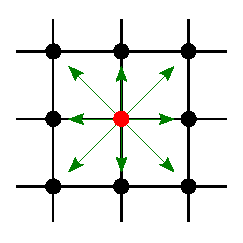
\includegraphics[width=0.95\textwidth]{colision}
        \caption{Colisi\'on}        
    \end{subfigure}
    \begin{subfigure}[t]{0.45\textwidth}
        \centering
        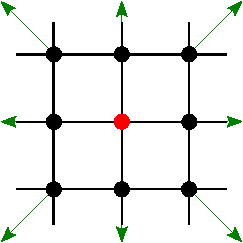
\includegraphics[width=0.95\textwidth]{streaming}
        \caption{Advecci\'on}        
    \end{subfigure}
    \caption{Representaci\'on esquem\'atica de las etapas principales de la soluci\'on de una \lbe{}.}
    \label{fig:lb_str_col}
\end{figure}
%\FloatBarrier

Durante el desarrollo de la etapa de colisi\'on es necesario involucrar a las variables macrosc\'opicas definidas a tiempo $t$, a trav\'es de la funci\'on de distribuci\'on o t\'erminos de fuente adicionales. Como esta informaci\'on es requerida numerosas veces durante un mismo paso de tiempo, es conveniente definir (computacionalmente) expl\'icitamente a las variables macrosc\'opicas y actualizar los valores de cada nodo s\'olo una vez por paso de tiempo. Con esta alternativa se construye el algoritmo general para la resoluci\'on de una \lbe{}, con los pasos que se resumen en el esquema de la \fig{fig:lb_algo}. Este mecanismo de resoluci\'on es el empleado en el desarrollo de esta tesis.
\begin{figure}[ht]
	\centering
	\begin{tikzpicture}[node distance = 2.5cm, auto]
    		% nodes
		\node [block] (init) {Inicializaci\'on \\ $\rho_i$, $\bm{u}_i$, \\ $f=f^{eq}(\rho_i,\bm{u}_i)$};
	    \node [block, below of=init] (col) {Colisi\'on \\ $f^* = \Omega(f)$};
	    \node [block, below of=col] (adv) {Advecci\'on};
	    \node [block, below of=adv] (cdb) {Condiciones de contorno};
	    \node [block, below of=cdb] (macro) {Actualizaci\'on \\ $\rho$, $\bm{u}$};
	    \node [decision, below of=macro] (decide) {?`Tiempo final?};
    	    \node [block, below of=decide, node distance=3cm] (fin) {Fin};
	    
	    % Edges
	    \path [line] (init) -- (col);
	    \path [line] (col) -- (adv);
	    \path [line] (adv) -- (cdb);
	    \path [line] (cdb) -- (macro);
	    \path [line] (macro) -- (decide);
	    \path [line] (decide) -- node {s\'i} (fin);
	    \path [line] (decide) -- +(-3,0) |- node [near start, sloped, above] {no. $t + \delta_t$} (col);	
	\end{tikzpicture}	
	\caption{Algoritmo LB general}
	\label{fig:lb_algo}
\end{figure}
\FloatBarrier



En la \fig{fig:lb_algo} se muestra un paso adicional (y fundamental) del algoritmo, que consiste en la implementaci\'on de condiciones de contorno. Despu\'es del paso de advecci\'on, los nodos ubicados sobre la frontera del dominio computacional contienen componentes que no pueden ser actualizadas, ya que no existen nodos vecinos en ciertas direcciones. En el caso de LB, esta informaci\'on puede reconstruirse con m\'etodos espec\'ificos para obtener el comportamiento hidrodin\'amico deseado, como restricciones en el valor de las variables macrosc\'opicas sobre paredes, condiciones peri\'odicas o de flujo saliente. En los cap\'itulos siguientes se aborda en detalle la incorporaci\'on de \'estos m\'etodos al algoritmo.

En su conjunto, LB es un m\'etodo que permite obtener la soluci\'on de ecuaciones de conservaci\'on sin necesidad de abordarlas directamente. La integraci\'on de la ecuaci\'on de Boltzmann mediante el m\'etodo de las caracter\'isticas conduce a una \lbe{} expl\'icita, y que presenta una convergencia de segundo orden en las coordenadas espaciales y temporal. Este resultado impacta significativamente en la eficiencia computacional del m\'etodo, ya que no es necesario resolver costosos sistemas de ecuaciones, como el correspondiente a la ecuaci\'on de Poisson para la presi\'on en los m\'etodos tradicionales. Por otro lado, el paso de advecci\'on simplifica el tratamiento de los t\'erminos convectivos no lineales de la ecuaci\'on de conservaci\'on de impulso. De esta manera se obtiene una t\'ecnica cuyo costo computacional global depende linealmente del n\'umero de nodos de la grilla, y con un algoritmo que facilita su implementaci\'on en sistemas de procesamiento distribuido. 

Sin embargo, esta aparente simplicidad tiene su precio. La mayor\'ia de los modelos LB presentan restricciones significativas de estabilidad, lo que limita su utilizaci\'on en la simulaci\'on de flujos con, por ejemplo, baja viscosidad. Si bien los operadores de colisi\'on MRT presentan rangos de estabilidad sensiblemente superiores a los BGK, a\'un sigue siendo insuficiente para determinadas aplicaciones. Por otro lado, el v\'inculo entre la \lbe{} y las ecuaciones macrosc\'opicas no siempre es sencillo de cuantificar. La expansi\'on de Chapman-Enskog est\'a basada en un an\'alisis asint\'otico, de modo que los resultados de las simulaciones pueden mostrar efectos de los t\'erminos de orden superior no considerados. Estas caracter\'isticas negativas deben ser consideradas al momento de aplicar la t\'ecnica, pero si su uso es factible, las limitaciones son ampliamente compensadas por la eficiencia y simplicidad del m\'etodo.


\section{Conclusiones}

El m\'etodo de lattice Boltzmann ha evolucionado hasta convertirse en una herramienta robusta y fiable para la simulaci\'on num\'erica de mec\'anica de fluidos. Desde un punto de vista formal, LB puede entenderse como un camino para resolver una ecuaci\'on de Boltzmann: en lugar de discretizar directamente aquellas ecuaciones de inter\'es, el m\'etodo propone transportar una funci\'on de distribuci\'on en una grilla regular, considerando que los momentos (en el espacio de fases) de esta \fdp{} est\'an asociados a las principales magnitudes hidrodin\'amicas de las ecuaciones macrosc\'opicas de inter\'es, como densidad, velocidad o temperatura. A trav\'es de t\'ecnicas de expansi\'on multiescala, como el an\'alisis de Chapman-Enskog, es posible verificar que una adecuada elecci\'on de grilla espacial, velocidades discretas del espacio de fases, y operador de colisi\'on, pueden ser combinadas adecuadamente para obtener la soluci\'on de ecuaciones de conservaci\'on de t\'ipicas de mec\'anica de fluidos. 